%%%%%%%%%%%%%%%%%%%%%%%%%%%%%%%%%%%%%%%%%%%%%%%%%%%
%% Capítulo 2: Iteración
%%%%%%%%%%%%%%%%%%%%%%%%%%%%%%%%%%%%%%%%%%%%%%%%%%%

Como hemos podido comprobar en el capítulo anterior, muchos de los fractales clásicos son generados repitiendo indefinidamente un proceso. Iteración es el proceso de repetir una y otra vez un método, ocasionalmente sobre el resultado de la aplicación anterior. Este procedimiento es muy útil en muchas disciplinas matemáticas. Por ejemplo, existen métodos numéricos basados en la iteración como el método de \textit{Jacobi} y \textit{Gauss-Seidel} para resolución de sistemas de ecuaciones lineales, el método de \textit{Newton-Raphson} para encontrar soluciones de ecuaciones, el método de \textit{Runge-Kutta} para resolución numérica de ecuaciones diferenciales, etc. Incluso en otras disciplinas como el aprendizaje automático los algoritmos de \textit{K-Means} para ``clustering'' o los métodos de generación de árboles de decisión en problemas de clasificación hacen uso de procesos iterativos. Esta metodología aplicada sobre el plano complejo y sobre ciertas funciones complejas será la que nos proporcionará nuestros primeros ejemplos de imágenes fractales.

\section{Iteración de funciones}
\begin{definicion}
    Consideramos una función $f:\C\longrightarrow\C$ y un punto $z\in\C$. La aplicación sucesiva de $f$ a $z$ -- \textit{i.e.} $z,f(z),f(f(z)), f(f(f(z))),\dots$ -- produce las \textbf{iteradas} de la función $f$ en el punto $z$. Al conjunto de dichas iteradas se le denomina \textbf{órbita} $O_f(z)$ de $f$ en $z$.
    $$
    O_f(z):=\left\lbrace z, f(z), f^2(z), \dots, f^n(z), \dots\right\rbrace.
    $$
    donde $f^n$ denota a $f\circ f^{n-1}$.
\end{definicion}

Lo siguiente es plantearse la posible convergencia de la sucesión $\{f^n(z)\}$. Para ello, y a partir de este momento nos ayudaremos del software \textcolor{blue}{\href{https://www.wolfram.com/mathematica/}{Mathematica®}} en su versión 12 (concretamente la versión 12.1)\footnote{Los códigos completos que generan cada una de las imágenes que se observan en este documento se pueden encontrar en \url{https://github.com/JAntonioVR/Geometria-Fractal/tree/main/Iteracion-y-Fractales}}. El comando \verb|NestList[f,z,n]| itera una función \verb|f|, comenzando en el punto \verb|z| un total de \verb|n| veces y devuelve una lista con los \verb|n| valores. 

Para saber qué ocurre a largo plazo podemos iterar un número grande de veces, fijémonos lo que ocurre si utilizamos $f(z):=z^2$ comenzando por $z_0=0.9$.

\begin{mmaCell}{Code}
  f[z_] := z^2;
  NestList[f, 0.9, 10]
\end{mmaCell}
\begin{mmaCell}{Output}
  \{0.9, 0.81, 0.6561, 0.430467, 0.185302, 0.0343368, \
  0.00117902, 1.39008*10^-6, 1.93233*10^-12, 3.73392*10^-24, \
  1.39421*10^-47\}
\end{mmaCell}

Como se puede observar, en cada iteración se acerca cada vez más a $0$, lo cual denotamos con $\{f^n(0.9)\}\rightarrow 0$. En este caso todos los valores eran reales, pero aprovechando la correspondencia de $\C$ con $\R^2$, de forma que un número complejo $z=x+y\cdot i\in\C$ se corresponde con el par $(x,y)\in\R^2$ podemos representar en el plano y de forma visual la tendencia de dichas sucesiones. Observemos los ejemplos de las imágenes \ref{fig:orbitas-C}.

\begin{figure}[ht]
    \centering
    \begin{tabular}{cc}
      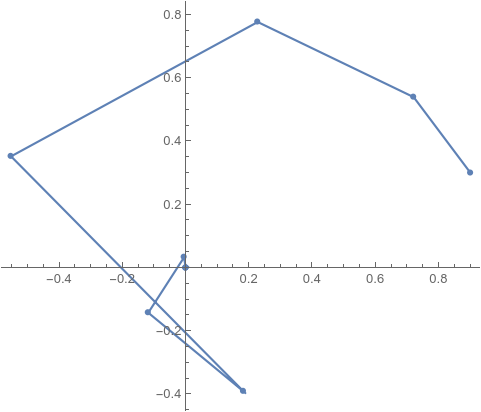
\includegraphics[scale=0.45]{./img/orbita-1.png} &   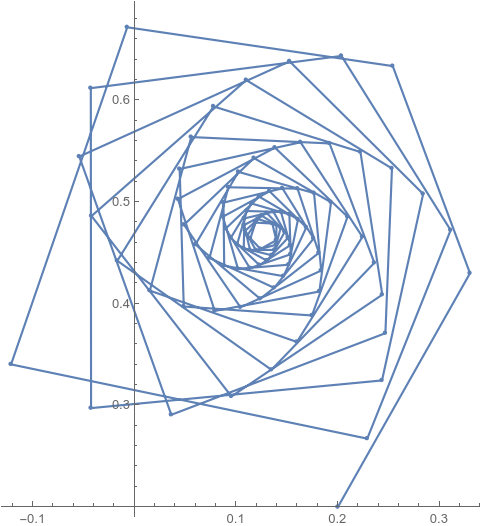
\includegraphics[scale=0.4]{./img/orbita-2.png} \\
    (a)$f(z)=z^2$ en $z=0.9+0.3i$ & (b) $f(z)=z^2+0.33+0.35$ en $z=0.2+0.2i$ \\[6pt]
    \end{tabular}
    \caption{Representación de dos órbitas en $\C$}
    \label{fig:orbitas-C}
\end{figure}

Los ejemplos expuestos hasta ahora son todos convergentes, pero esto no es siempre así. Nuestro objetivo ahora es poder conocer el comportamiento a largo plazo de la órbita de una función y un punto dados. 

\subsection{Convergencia a un punto fijo}
\label{subsection:convergencia-punto-fijo}

Fijémonos que en el ejemplo anterior si en lugar de tomar $z_0=0.9$ hubiésemos tomado cualquier valor con $|z_0|<1$ la convergencia habría sido igualmente a $0$, pues elevamos al cuadrado cada vez números más pequeños. Justo al contrario ocurre si $|z_0|>1$, en cuyo caso la sucesión diverge. Por último, en caso de que $|z_0|=1$, esto es, $z_0\in S^1$, la sucesión $\{f^n(z_0)\}$ nunca saldrá de $S^1$, siendo este el conjunto que delimita la frontera entre el conjunto de puntos cuya sucesión converge o diverge. En particular, $f^n(-1)=f^n(1)=1\ \ \forall n\in\N$, por lo que $z=1$ es un punto fijo de $f$, es decir, $f(z)=z$. 

Nos interesa particularmente saber qué sucesiones de iteradas convergen y a qué elemento convergen. En este sentido \textit{Stephan Banach} demostró uno de los resultados más útiles y vigentes del análisis funcional:

\begin{teorema}[Punto fijo de Banach]
    \label{th:punto-fijo}
    Sea $X$ un espacio métrico completo y $f:X\longrightarrow X$ una aplicación contractiva. Entonces $f$ tiene un único punto fijo. Además, la sucesión de iteradas $\{f^n(x_0)\}$ converge a dicho punto fijo para cualquier $x_0\in X$. 
\end{teorema}
\begin{proof}
    Probaremos primero la existencia:

    Sea $x_0\in X$ y sea la sucesión de iteradas $\{x_n\}=\{f^n(x_0)\}$. Por ser $f$ contractiva, llamamos $K<1$ a su constante de Lipschitz. Probaremos por inducción que $d(x_n,x_{n+1})\leq K^n d(x_0,x_1) \ \ \forall n\in\N$.
    El caso base es cierto pues $d(x_1,x_2)=d(f(x_0),f(x_1))\leq K d(x_0,x_1)$. Si suponemos que la hipótesis es cierta para cierto $n$, tenemos que
    $$
    d(x_{n+1},x_{n+2})=d(f(x_n),f(x_{n+1}))\leq K d(x_n,x_{n+1})\leq K^{n+1}d(x_0,x_1).
    $$
    Ahora, para $n,r\in\N$:
    \begin{eqnarray*}
        d(x_n,x_{n+r}) & \leq & \sum_{j=0}^{r-1}d(x_{n+j},x_{n+j+1}) \leq d(x_1,x_0)\sum_{j=0}^{r-1}K^{n+j} \leq K^n d(x_0,x_1)\sum_{j=0}^{\infty} K^j \\
        & = & \frac{d(x_0,x_1)K^n}{1-K}.
    \end{eqnarray*}
    Dado $\varepsilon>0$, como $\{K^n\}\rightarrow 0$, existe un $m\in\N$ tal que para $n>m$ se tiene que $d(x_0,x_1)K^n<\varepsilon(1-K)$. Si ahora tomamos dos naturales $p,q\geq m$ con $p<q$, aplicando la desigualdad anterior tomando $n=p$ y $r=q-p$ obtenemos que:
    $$
    d(x_p,x_q) = d(x_n, x_{n+r}) \leq \frac{d(x_0,x_1)K^n}{1-K} < \varepsilon
    $$
    de donde deducimos que $\{x_n\}$ es una sucesión de Cauchy, y como $X$ es completo, tenemos que $\{x_{n+1}\}=\{f(x_n)\}=\{f^n(x_0)\}\rightarrow x\in X$. Pero $f$ es continua, por lo que si $\{x_n\}\rightarrow x$, necesariamente $\{f(x_n)\}\rightarrow f(x)$, por lo que $f(x)=x$.

    Para probar la unicidad, suponemos que $y\in X$ es otro punto fijo de $f$, por lo que $d(x,y) = d(f(x),f(y))\leq K d(x,y)$. Tomando el primero y el tercer miembro de la desigualdad deducimos que $(1-K)d(x,y)\leq 0$, luego $d(x,y)=0$.
\end{proof}

Este teorema unido a que sabemos que $\C$, y por tanto todos sus subconjuntos cerrados, es completo, nos permite asegurar convergencia de las sucesiones $f^n(x_0)$ a un punto fijo para cualquier $x_0$ siempre que dicha función sea contractiva.

\subsection{Velocidad de convergencia}

Si recordamos el teorema del punto fijo de Banach (teorema \ref{th:punto-fijo}), que nos decía que las funciones contractivas en un espacio métrico completo admiten un único punto fijo, el cual se puede hallar iterando la función. Recordemos que dada una función $f:\C\longrightarrow\C$ contractiva, esta cumple que $|f(z_1)-f(z_2)|\leq K|z_1-z_2|\ \ \forall z_1,z_2\in\C$, siendo $0<K<1$ la constante de Lipschitz de $f$, nombrada en este caso la constante de contractividad. Fijémonos que, si iteramos $n$ veces la función $f$
\begin{eqnarray*}
    |f^n(z_0)-f^{n-1}(z_0)| & \leq & K|f^{n-1}(z_0)-f^{n-2}(z_0)| \\
    & \leq & K^2 |f^{n-2}(z_0)-f^{n-3}(z_0)| \\
    & \leq\cdots\leq&K^{n-1}|f(z_0)-z_0|
\end{eqnarray*}
por lo que en realidad la constante $K$ define de forma genérica la velocidad de convergencia en términos de la función. Cuanto más cercana a $0$, más rápida será la convergencia al punto fijo. Sin embargo, vemos que realmente también depende de la condición inicial fijada, y es este el aspecto que explotaremos para obtener imágenes fractales. 

En los casos que tengamos asegurada la convergencia, es interesante saber cuántas iteraciones son necesarias en cada punto para saber si hemos alcanzado el valor al que converge la sucesión. Este alcance se toma como aproximado, pues generalmente nunca se llega a alcanzar el punto fijo, tan solo podemos reducir la diferencia tanto como queramos. En este sentido, \textit{Mathematica} tiene dos comandos útiles:

\begin{itemize}
    \item \verb|FixedPointList[f,expr]| genera una lista de valores resultantes de aplicar \verb|f| a \verb|expr| repetidamente hasta que los dos últimos valores no cambian. Para parametrizar la precisión en la proximidad de los valores podemos utilizar el argumento opcional \verb|SameTest|\footnote{Más información en la documentación oficial \url{https://reference.wolfram.com/language/ref/FixedPointList.html}}.
    \item \verb|FixedPoint[f,expr]| hace lo mismo pero produce como salida únicamente el valor último producido.
\end{itemize}

El siguiente código muestra un ejemplo de uso:

\begin{mmaCell}{Code}
  f[z_] = z/2 + 1/z;
  FixedPointList[f, 0.75 + 0.1 I, SameTest -> (Abs[#1 - #2] < 10^-4 &)]
  FixedPoint[f, 0.75 + 0.1 I]
\end{mmaCell}
\begin{mmaCell}{Output}
  \{0.75 + 0.1 I, 1.68504 - 0.124672 I, 1.43275 - 0.0186668 I, \
  1.41421 - 0.000241452 I, 1.41421 - 2.45537*10^-10 I, \
  1.41421 + 3.57849*10^-18 I\}
\end{mmaCell}
\begin{mmaCell}{Output}
  1.41421 + 0. I
\end{mmaCell}

Y a partir de la longitud de la lista que nos devuelve \verb|FixedPointList|, es decir, con el sencillo comando \verb|Length[FixedPoint[f,x]]| podemos medir la velocidad de convergencia de cada punto.

\section{El método de Newton y cuencas de atracción}

Gracias a la iteración y al estudio de la convergencia de las sucesiones que definen las órbitas, podemos definir muchos métodos numéricos que nos ayuden a resolver numéricamente problemas que de forma teórica o analítica serían difíciles de abordar. Entre estos está el conocido \textbf{método de Newton}. Este es un procedimiento iterativo que nos permite adivinar con cierta precisión donde se anula una función derivable (al menos en un entorno de la raíz), pudiendo así utilizarlo como herramienta para la resolución de ecuaciones. Existen varias y distintas versiones del método de Newton, siendo la más sencilla la que busca las raíces de una función real de variable real $f:\R\longrightarrow\R$, conociéndose también en este caso como \textit{método de Newton-Raphson}. Además, hay una generalización para aplicaciones $f:\R^n\longrightarrow\R^n$, la cual se apoya en la inversa del operador diferencial. Sin embargo, nosotros estamos trabajando con funciones complejas $f:\C\longrightarrow\C$, que aunque $\C$ y $\R^2$ sean isomorfos, la dinámica es distinta, pues si la función compleja es suficientemente buena, podemos usar su derivada $f'(z)$ y no el operador diferencial (véase \cite{Dubeau-Gnang}). 

Recordemos que dada una ecuación $f(z)=0$ para cierta función compleja y analítica $f:\C\longrightarrow\C$, el método de Newton itera la función
\begin{equation}
    \label{eq:metodo-Newton}
    N_f(z)=z-\frac{f(z)}{f'(z)}
\end{equation} 
comenzando por un punto $z_0$ cercano a la raíz. Es decir, calcula la sucesión $\{z_n\}$ definida como $z_{n+1}=N_f(z_n) \ \forall n\in\N$, la cual aplicando el teorema \ref{th:punto-fijo} podemos deducir que converge a un punto $a\in\C$ que verifica $f(a)=0$ siempre que $f'(a)\not= 0$. Para mayor detalle acerca de la convergencia local ver \cite[Capítulo 7]{Ostrowski} y \cite[Sección 5.4]{Atkinson}.

Sin embargo, en muchas ecuaciones, comenzando por las polinómicas de grado mayor que 1, existen varias soluciones distintas, pero el método de Newton converge sólo a una de ellas, dependiendo de qué $z_0$ fijemos. Nuestro objetivo ahora se sitúa en discernir, para cada punto $z_0$ del plano, a qué solución de la ecuación $f(z)=0$ converge la sucesión $\{z_n\}$ dada por el método de Newton utilizando a $z_0$ como semilla. En las siguientes secciones veremos algunos ejemplos de esta distinción y su utilidad, llegando a las primeras imágenes fractales generadas por iteración.

\begin{ejemplo}
\label{ejemplo:cuencas-1}
Consideramos la función compleja $f:\C\longrightarrow\C$ dada por $f(z)=z^2-1$, la cual tiene dos raíces: $1$ y $-1$, las dos raíces cuadradas de 1. Una forma sencilla de comprobar a qué raíz converge cada sucesión utilizando como semilla cada $z_0\in\C$ es asociando un color a cada punto del plano dependiendo de la raíz a la que converja y pidiendo a \textit{Mathematica} que coloree el plano complejo siguiendo este criterio.

\begin{mmaCell}{Code}
  iteracionN = #2 - #1[#2]/Derivative[1][#1][#2] &;
    newtonArgumento = 
    Compile[{{z, _Complex}}, 
    Arg[FixedPoint[iteracionNR[f, #] &, z, 50]]];
    
  DensityPlot[newtonArgumento[x + I*y], {x, -2, 2}, {y, -2, 2}, 
    PlotPoints -> 100, Mesh -> False, ColorFunction -> "Rainbow"] 
\end{mmaCell}

\begin{figure} [ht]
\centering
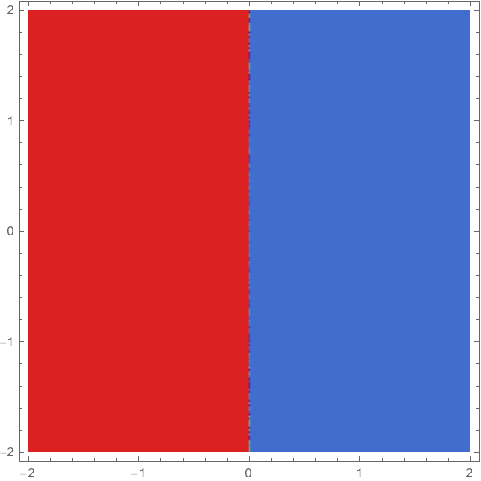
\includegraphics[scale = 0.4]{img/cuencas-1.png}
\caption{Cuencas de atracción de $f(z)=z^2-1$.}
    \label{fig:cuencas-1}
\end{figure}

Produciendo como resultado la imagen \ref{fig:cuencas-1}. La forma de deducir a qué raíz converge cada sucesión consiste en evaluar los argumentos de los valores a los que se acerca la misma. Como podemos ver, y teniendo en cuenta que la imagen solo grafica el intervalo $[-2,2]\times[-2,2]$ y un número finito de puntos\footnote{El número de puntos que se grafica se puede parametrizar con el argumento opcional ``PlotPoints'' de las funciones ``Plot''. A mayor valor mayor calidad de imagen y resolución, pero mayor tiempo de ejecución.} la sucesión cuya semilla es un punto perteneciente al semiplano abierto de la derecha converge a la raíz $1$. Por otro lado, si la sucesión comienza con un complejo del semiplano abierto de la izquierda, entonces esta converge a la raíz $-1$. Apoyándonos en este ejemplo, definimos el siguiente concepto.
\end{ejemplo}


\begin{definicion}[Cuenca de atracción]
    Definimos como \textbf{cuenca de atracción} de una raíz $a\in\C$ de una función compleja $f:\C\longrightarrow\C$ (\textit{i.e.} $f(a)=0$), y denotamos como $A(a)$ al conjunto de puntos $z_0\in\C$ tales que la sucesión $\{z_n\}$ dada por $z_{n+1}=N_f(z_n)$ converge a $a$ utilizando a $z_0$ como primer valor de la sucesión. 
\end{definicion}

En muchas de las funciones que trataremos ocurre que existen distintas cuencas de atracción y la distinción sobre a cuál de ellas pertenece cada punto del plano complejo es la que nos permitirá graficar imágenes fractales. Si aplicamos el mismo procedimiento antes descrito en el ejemplo \ref{ejemplo:cuencas-1} con otras funciones encontramos las imágenes \ref{fig:cuencas-raiz}.

\begin{figure}[ht]
    \centering
    \begin{tabular}{ccc}
      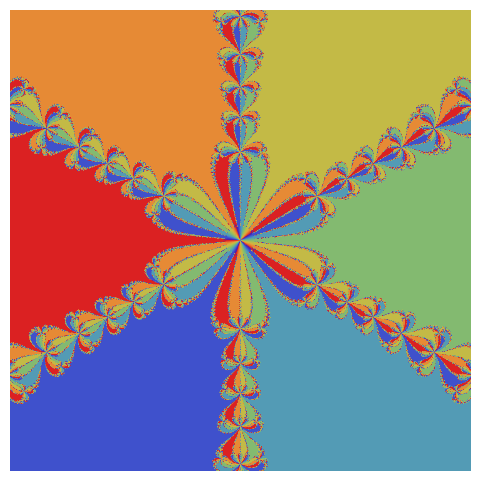
\includegraphics[scale=0.33]{img/cuencas-color-1.png} &   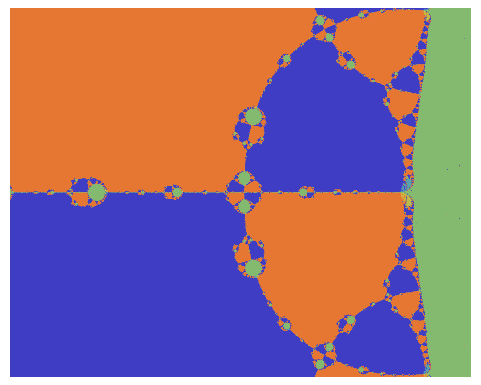
\includegraphics[scale=0.31]{img/cuencas-color-2.png} &   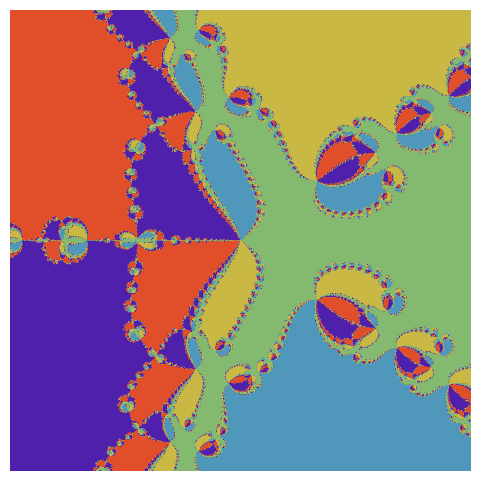
\includegraphics[scale=0.33]{img/cuencas-color-3.png} \\
    (a) $f(z)=z^6-1$ & (b) $f(z)=z^3-3^z$ & (c) $f(z)=z^5-z^3+z^2-4$ \\[6pt]
    \end{tabular}
    \caption{Cuencas de atracción de distintas funciones coloreadas.}
    \label{fig:cuencas-raiz}
\end{figure}

En estas imágenes podemos ahora sí ver los primeros ejemplos de estructuras fractales producidos por la iteración. Observemos que las sucesiones de dos puntos muy próximos pueden converger a raíces distintas, por lo que este es un ejemplo de \textit{caos matemático}: pequeñas variaciones en las condiciones iniciales conducen a comportamientos muy diferentes. Además, en lugar de colorear el plano según la raíz a la que converja la sucesión también podemos fijarnos en la velocidad de convergencia. Esto es, asociar a cada punto del plano un color dependiendo del número de iteraciones necesarias para converger a la raíz. En este sentido, podemos revisitar las imágenes \ref{fig:cuencas-raiz} y en función de la velocidad de convergencia de las sucesiones utilizar un color distinto. El código necesario es el siguiente y los resultados se pueden observar en las imágenes \ref{fig:cuencas-velocidad}:

\begin{mmaCell}{Code}
  newtonVelocidad = Compile[{{z, _Complex}}, 
    Length[FixedPointList[iteracionN[f, #] &, z, 50]]];
    
  DensityPlot[newtonVelocidad[x + I*y], {x, -2, 2}, {y, -2, 2}, 
    PlotPoints -> 200, Mesh -> False, ColorFunction -> GrayLevel]
\end{mmaCell}

donde se puede cambiar el valor de \verb|f|, la región del plano \verb|{x, -2, 2}, {y, -2, 2}| o el valor del argumento \verb|ColorFunction| para obtener distintas imágenes.

\begin{figure}[ht]
    \centering
    \begin{tabular}{ccc}
      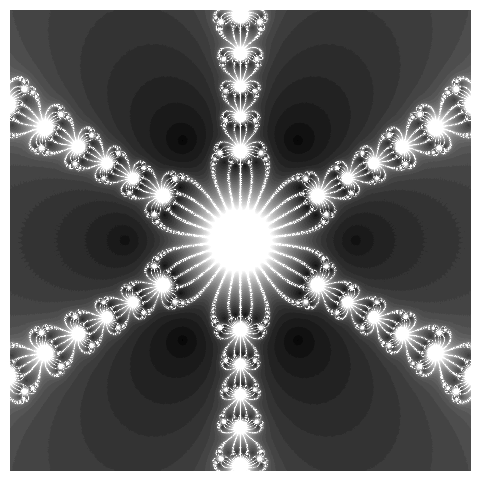
\includegraphics[scale=0.33]{img/cuencas-velocidad-1.png} &   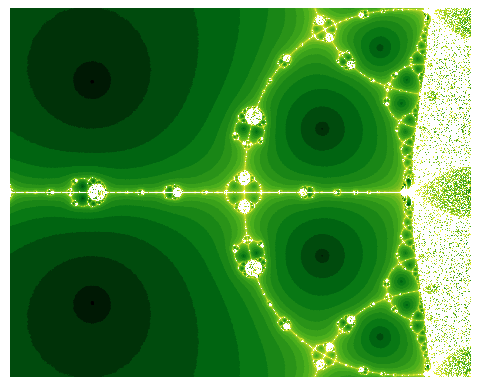
\includegraphics[scale=0.31]{img/cuencas-velocidad-2.png} &   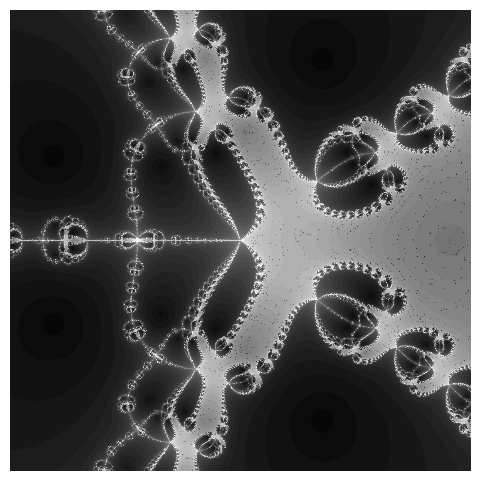
\includegraphics[scale=0.33]{img/cuencas-velocidad-3.png} \\
      (a) $f(z)=z^6-1$ & (b) $f(z)=z^3-3^z$ & (c) $f(z)=z^5-z^3+z^2-4$ \\[6pt]
    \end{tabular}
    \caption{Evaluación de la velocidad de convergencia en cada punto}
    \label{fig:cuencas-velocidad}
\end{figure}

Podemos jugar con estos parámetros como son la función a representar \verb|f|, la región del plano que queremos visualizar \verb|{x, -2, 2}, {y, -2, 2}| o el valor del argumento \verb|ColorFunction| para obtener distintas imágenes de diferentes colores.

\subsection{Autosimilaridad}
\label{subsection:autosimilaridad}

Consideramos ahora la representación de las cuencas de atracción de la función compleja $f(z)=z^3-1$, que podemos ver en la imagen \ref{fig:cuencas-autosimilaridad}

\begin{figure} [ht]
\centering
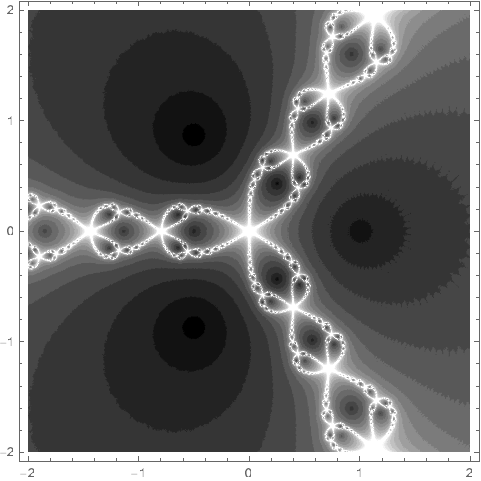
\includegraphics[scale = 0.5]{img/cuencas-autosimilaridad.png}
\caption{Cuencas de atracción de $f(z)=z^3-1$}
    \label{fig:cuencas-autosimilaridad}
\end{figure}

\newpage

Fijémonos además que si hacemos \textit{zoom} en ciertas partes de la imagen, es decir, representamos una región más pequeña, encontramos estructuras que son iguales independientemente del zoom que se aplique. En la figura \ref{fig:detalles} podemos ver distintos detalles de la figura \ref{fig:cuencas-autosimilaridad}, cada una es una ampliación de la anterior, y podemos ver como esa estructura se repite en todas las escalas.


\begin{figure}[ht]
    \begin{tabular}{ccc}
      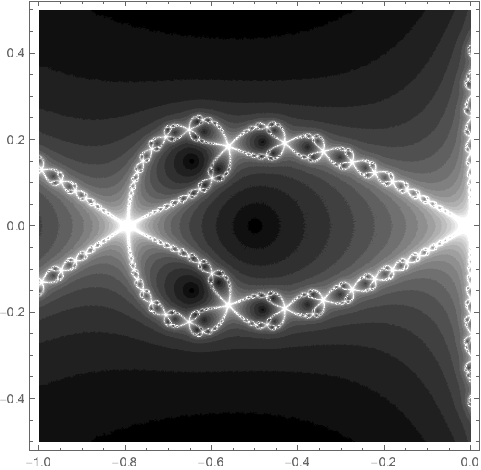
\includegraphics[scale=0.33]{./img/detalle-1.png} &   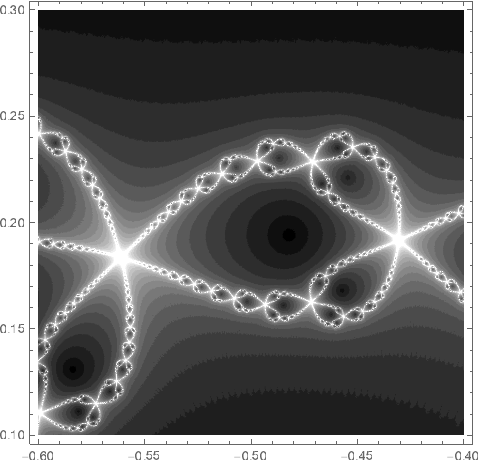
\includegraphics[scale=0.33]{./img/detalle-2.png} &   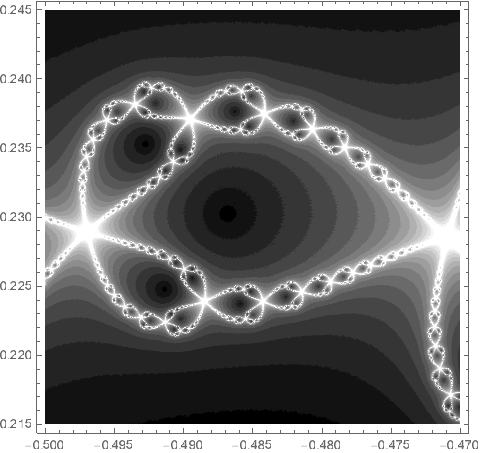
\includegraphics[scale=0.33]{./img/detalle-3.png} \\
    (a) $[-1,0]\times[-0.5,0.5]$ & (b) $[-0.6,-0.4]\times[0.1,0.3]$ & (c) $[-0.5,-0.47]\times[0.215,0.245]$ \\[6pt]
    \end{tabular}
    \caption{Diferentes regiones ampliadas de la figura \ref{fig:cuencas-autosimilaridad}}
    \label{fig:detalles}
\end{figure}

Este aspecto es el que realmente nos define la naturaleza fractal de las cuencas de atracción, pues aunque las imágenes no son objetos totalmente autosimilares en el sentido de la definición \ref{def:autosimilaridad} si que contienen regiones que sí lo son, como es el caso que acabamos de describir.